\chapter{Event Reconstruction and Selection}
\section{Reconstruction}
\subsection{Tracking}
\label{sec:track_recon}

\subsubsection{Hit Reconstruction}
\label{sec:svt_hit_recon}

\subsubsection{Track Finding and Refit}
\label{sec:track_finding_refit}
track finding

GBL refit

\subsection{Vertexing}
\label{sec:vertex_recon}
Pairs of tracks are vertexed using a fast vertex fit that finds the best-fit vertex position and track parameters based on the track parameters and covariance matrices, and optional additional vertex constraints \cite{billoir_fast_1992}.

The HPS vertex reconstruction uses constraints on the $x$, $y$, and $z$ location of the vertex.
All constraints are limited by the vertex resolutions in those directions; the $x$ and $y$ constraints are limited by the beamspot size, and the $z$ constraint is limited by knowledge of the target position, but these are all smaller than the vertex resolutions.
%Three types of constraints are used, all using knowledge about the target and/or beamspot.
The ``$z$-constrained'' fit requires that the vertex be consistent with the $z$ location of the target.
The ``target-constrained'' fit requires that the vertex be consistent with the $z$ location of the target, and with the $x$ and $y$ location of the beam spot.
The ``beamspot-constrained'' fit requires that the vertex position and momentum are such that the vertex momentum points back to the beamspot at the target $z$.

\subsection{Clustering}
\label{sec:clustering}

\subsection{Track-Cluster Matching}
\label{sec:matching}
\section{Tracker Performance and Alignment}
\subsection{Internal Alignment}
\label{sec:internal_alignment}
millepede
\subsection{Elastic Electrons}
\label{sec:target_z}
\subsection{M{\o}ller Electrons}
\label{sec:mollers}

\section{\texorpdfstring{$e^+e^-$}{e+e-} Selection Cuts}
\label{sec:event_selection}
After reconstruction, all possible $e^+e^-$ pairs in the event are tested against a set of cuts.
There is no explicit requirement that the electron and positron be the pair of particles that caused the trigger.
There is also no fiducial requirement, since the inner edge of the detector acceptance is key for sensitivity to low-mass heavy photons.
The base selection is intended to remove accidental coincidences from the pair sample; the pair sample should contain only events where the electron and positron originate in the same interaction.

The ``pairs-1'' trigger is the HPS physics trigger, described in Section \ref{sec:trigger_cuts}.
It is tuned to accept $e^+e^-$ pairs, and is the overwhelming majority of the event rate (16.6 kHz out of 19 kHz).

The electron and positron are required to be in opposite halves of the detector: this cut is implemented as a requirement that the $y$-coordinates of the two clusters have opposite signs.
The trigger requires a top-bottom coincidence, so repeating the requirement as an event selection cut does not reduce the efficiency.
This cut eliminates any possibility of confusion in the track or cluster reconstruction, since the hits from the electron and positron are guaranteed to be well separated.
%A heavy photon can have enough transverse momentum that both decay products land in the same half of the detector, but the rate is low.

Track-cluster matching is important for two reasons: the cluster time resolution is better than the track time resolution, and track-cluster matching eliminates many misreconstructed tracks.
Two checks are done on the quality of the track-cluster matching for both particles.
First, a cut is made on the $\chi^2$ of the track-cluster match; this is a requirement on the distance between the cluster position and the track extrapolation to the ECal.
Second, a cut is made on the track-cluster time difference.
Since the track and cluster times are referenced differently (the track time is relative to the trigger time, and the cluster time is relative to the start of the ECal readout window), a constant offset of 43 ns is subtracted.

Three more simple cleanup cuts are applied.
A loose track quality cut is applied on the $\chi^2$ of each GBL fit; this is only meant to reject very poor track fits.
Elastically scattered electrons with $p(e^-)\approx E_{beam}$ are the main pileup background in the tracker, and are rejected with a maximum momentum requirement on electrons.
A momentum sum cut rejects pairs with a momentum sum too far in excess of $E_{beam}$; this further reduces the rate of random coincidences with elastic electrons.

The last cleanup cut is a cut on the cluster time difference.
This selects time coincidences.
The track time difference could be used similarly, but the cluster time resolution is better.

Finally, a ``radiative cut'' is applied for heavy photon analyses.
This is a minimum requirement on the momentum sum, at $0.8E_{beam}$.
As shown in Section \ref{sec:signal_kinematics}, most heavy photons and radiative tridents are produced with energy near $E_{beam}$; the radiative cut keeps most of these and rejects the Bethe-Heitler tridents that dominate at low momentum.

\begin{table}[ht]
    \begin{center}
        \begin{tabular}{lc}   
            \hline \hline
            Trigger type & ``pairs-1'' trigger \\
            Top-bottom requirement & $\sign(y_{cl}(e^-))\neq\sign(y_{cl}(e^-))$ \\
            Track-cluster matching (position) & $\chi^2_{match}<10$ \\
            Track-cluster matching (time) & $|t_{cl}-t_{trk}-43|<4$ ns \\
            Track quality & $\chi^2_{trk}<50$ \\
            Elastics cut & $p(e^-)<0.75E_{beam}$ \\
            Momentum sum cut & $p_{tot}(e^+e^-)<1.15E_{beam}$ \\
            Cluster time coincidence & $|t_{cl}(e^-)-t_{cl}(e^+)|<2$ ns \\
            Radiative cut & $p_{tot}(e^+e^-)>0.8E_{beam}$ \\
            \hline \hline
        \end{tabular}
        \caption{Base pair selection cuts for HPS.}
        \label{tab:basic_cuts} 
    \end{center}
\end{table}

\subsection{Tuning Cuts}
The cuts are tuned on the data, using the cluster time difference to separate ``good'' and ``bad'' events.
Pairs with large cluster time difference ($|t_{cl}(e^-)-t_{cl}(e^+)|>3$ ns) are accidental coincidences; pairs with small cluster time difference ($|t_{cl}(e^-)-t_{cl}(e^+)|<1$ ns) are dominated by true time coincidences.
An effective cut should reject pairs with large cluster time difference, and not pairs with small cluster time difference.

Figure \ref{fig:basecut_performance} shows the effect of the cuts on the distribution of cluster time differences.
This distribution is the sum of the distributions of true coincidences and random coincidences.
The distribution of true coincidences is a single peak with shape determined by the time resolution, and the distribution of random coincidences is the sum of multiple peaks spaced by the 2 ns beam period, with a slowly varying envelope shaped by the efficiencies of the trigger and track reconstruction.
If (as is the case for all cuts shown in the figure) a cut is not directly sensitive to the cluster time difference, and yet suppresses the outer peaks more than the central peak, it must be rejecting random coincidences.
%Each cut rejects more of the out-of-time events than the in-time events.
%Since the cluster time coincidence cut is the only cut that uses the cluster time difference, this implies that the fraction of accidental coincidences in the central peak decreases

The cluster time coincidence cut is applied after the other cuts, and selects only the central peak.
The rate of random coincidences contaminating the central peak can be estimated from the outer peaks: the fraction of random coincidences after the event selection cuts is roughly 1.5\%.

\begin{figure}[ht]
\begin{center}
    \includegraphics[width=0.6\textwidth,page=2,angle=-90]{recon/figs/basecutplots}
\end{center}
    \caption{Cumulative effect of the different pair selection cuts on pair-1 events passing the top-bottom requirement and radiative cuts.
    The ratio of out-of-time to in-time events (outer peaks to central peak) decreases as cuts are applied (going from the black to the magenta distributions).
    }
    \label{fig:basecut_performance}
\end{figure}

\section{Data Normalization}
\label{sec:luminosity}
Since the expected rate of heavy photons can be normalized to the data, a precise measurement of the integrated luminosity is not critical to the analysis.
Normalizing the data to the integrated luminosity is still essential for understanding the detector efficiencies and comparing the data to the cross sections of known processes.

The luminosity is the product of the beam current, target thickness, and experiment livetime.
The beam current is measured by a Faraday cup, as described in Section \ref{sec:beamline}.

\begin{equation}
\end{equation}
The beam current and trigger livetime

\subsection{Rate Comparison with Monte Carlo}
\label{sec:rates}